\chapter{Úvod}

Stavebnice \lego{ }je pravděpodobně nejznámější a nejprodávanější stavebnicí. 
Ve své nabídce mají i robotický set, který označují jako \legoM. 
Dle oficiálních údajů se jedná o historicky nejprodávanější set z celé nabídky firmy \cite{legoMindstorms_GizmodoSalesStatistic}. 
Jedná se o jeden z hlavních důvodů, proč se tato práce věnuje právě této stavebnici. 

Z výše uvedených důvodů se jedná pravděpodobně o nejdostupnější robotickou stavebnici na světě (pokud pomineme platformu \arduino, která je ovšem zaměřena na lidi, kteří se nebojí elektroniky, elektronický obvodů, složitějších návrhů konstrukce, atd.).

\begin{figure}[h]
 	\centering
	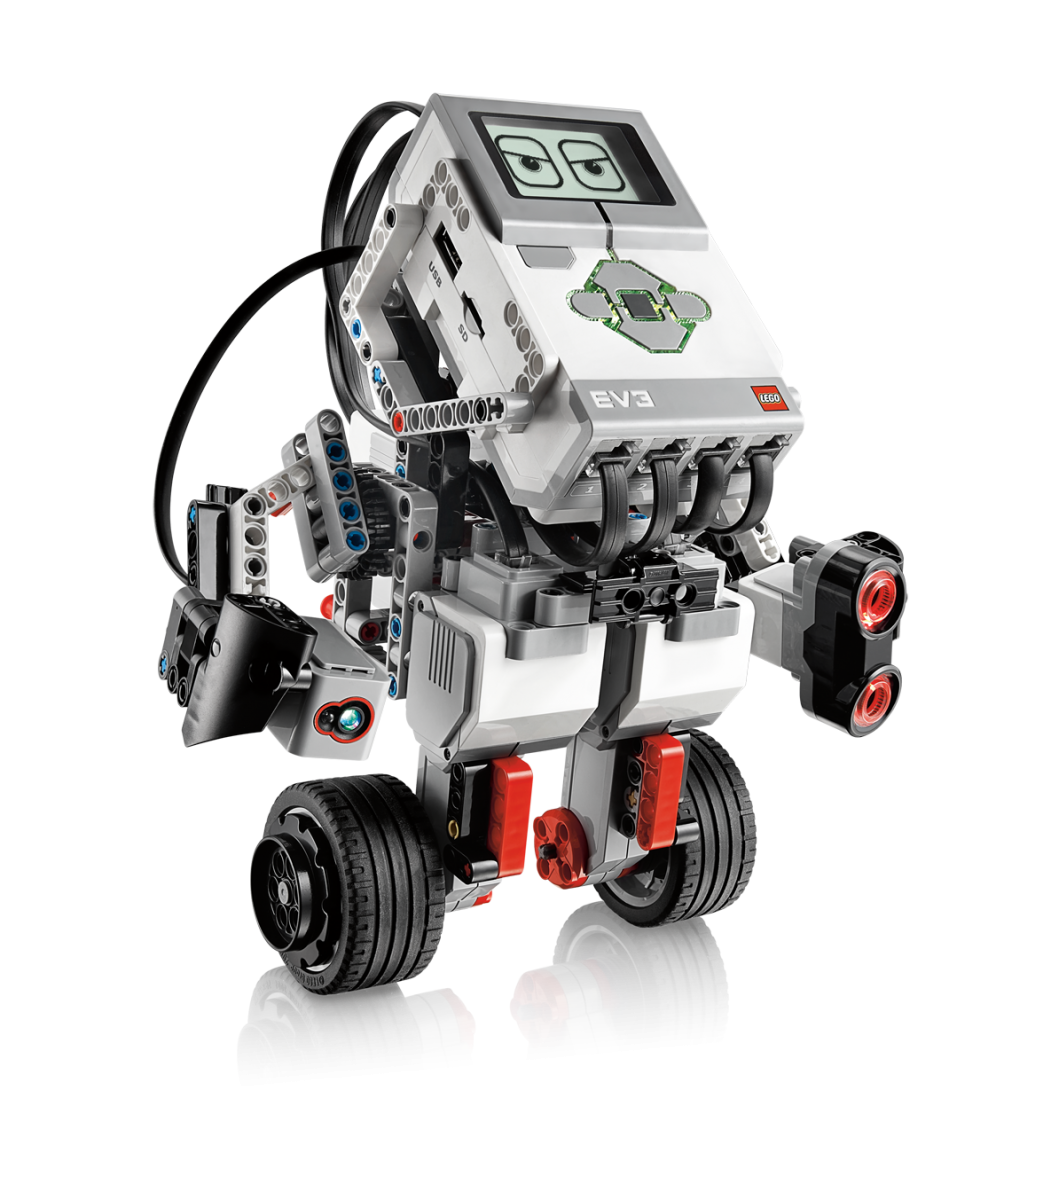
\includegraphics[width=250px]{images/lego-mindstorms-ev3_Robotics-for-Kids.png}
		\caption[\legoEV{ }-- samobalancující robot]{\legoEV{ }-- samobalancující robot\protect\footnotemark}
	\label{fig:lego-mindstorms-ev3_Robotics-for-Kids}
\end{figure}


\footnotetext{Zdroj: \url{https://www.bermotech.com/training/coding-for-teenagers-and-children/y-robotics-with-lego-mindstorm-ev3/}}

\begin{figure}[h]
 	\centering
	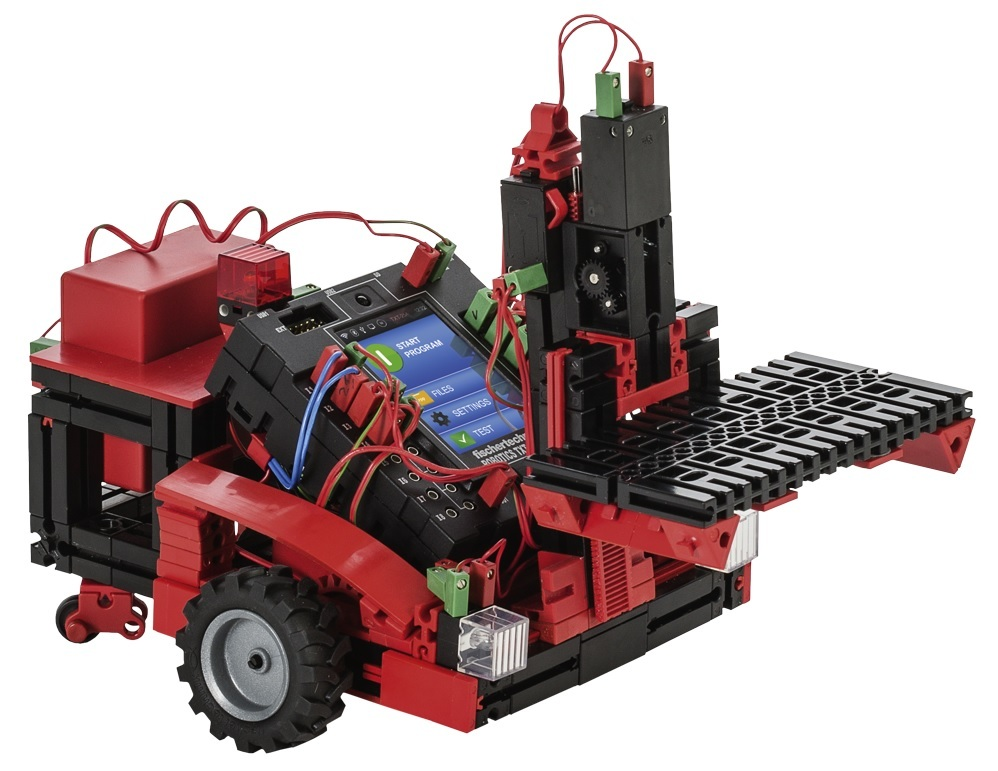
\includegraphics[width=250px]{images/fischertechnik_ROBO-TX-Explorer_02.jpg}
		\caption[Fischertechnik -- ROBO TX Explorer]{Fischertechnik -- ROBO TX Explorer\protect\footnotemark}
	\label{fig:fischertechnik_ROBO-TX-Explorer}
\end{figure}

\footnotetext{Zdroj: \url{http://www.helago-cz.cz/eshop-519143-workstation-robo-tx-training-lab-tx-explorer-146560.html}}

Existují i mnoho podobných stavebnic \cite{intorobotics_BestAlternativesToLegoMindstormsKits}. 
Lze se například setkat se stavebnicí \fischerT, která nabízí podobné robotické sety jako \lego{ }\cite{fischertechnik_ROBOTICS}. 
Uživateli ale poskytuje rozsáhlejší pohled do elektroniky a fungování jednotlivých modulů. 
Umožňuje také relativně snadno přidat vlastní moduly.
Zároveň stále zachovává jednoduché grafické programovací prostředí. 
\FischerT{ }ovšem není tak rozšířen, jako \legoM, protože ačkoliv nabízí v některých ohledech více funkcí, zároveň klade větší nároky na uživatele, je i podstatně dražší (základní set \cite{fischertechnik_HelagoEshop_ROBOTICS-TXT-COMPETITION-SET} stojí cca. dvakrát tolik co \legoEV{ Základní souprava}~\cite{lego_eduxeEshop_CoreSet}) a nemá takový věhlas a značku jako \lego.

% figure + footnote -> minipage 
%src: http://www.tex.ac.uk/FAQ-ftncapt.html
%\begin{figure}[h]
%\begin{minipage}{\textwidth}
%  	\centering
% 	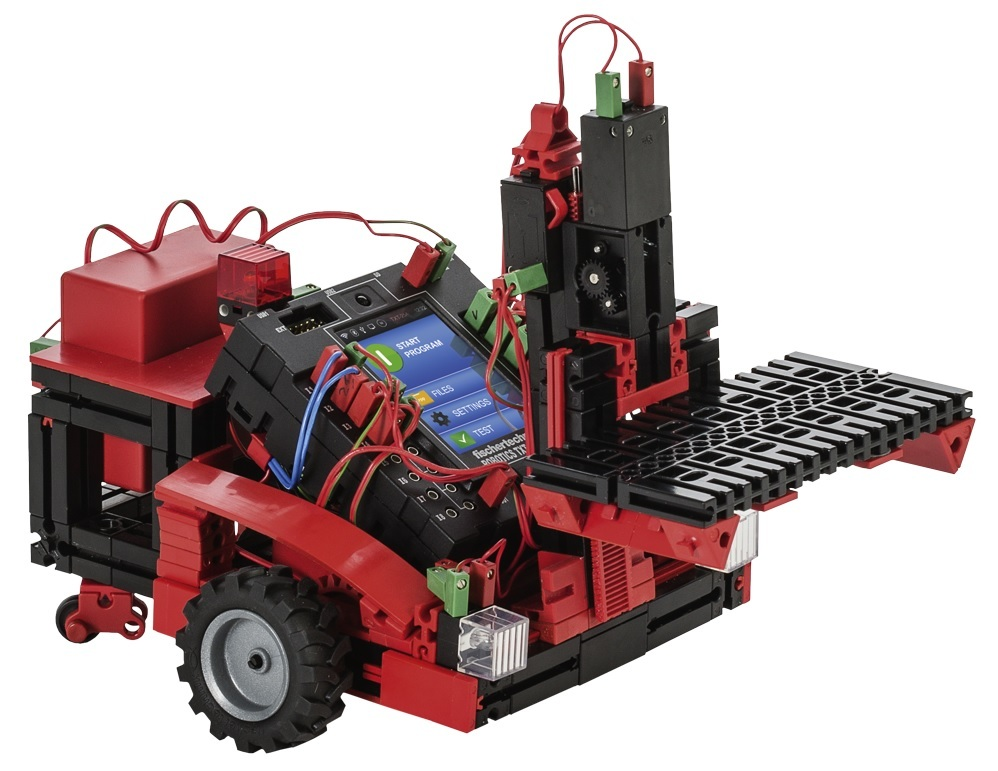
\includegraphics[width=300px]{images/fischertechnik_ROBO-TX-Explorer_02.jpg}
% 	\caption[Fischertechnik - ROBO TX Explorer]{Fischertechnik - ROBO TX Explorer \footnote{Zdroj: \url{http://www.helago-cz.cz/eshop-519143-workstation-robo-tx-training-lab-tx-explorer-146560.html}}
%\end{minipage}
%\end{figure}

% figure + footnote -> afterpage
% src: http://tex.stackexchange.com/questions/10181/using-footnote-in-a-figures-caption
%\afterpage{
%	\begin{figure}[h]
%	 	\centering
%		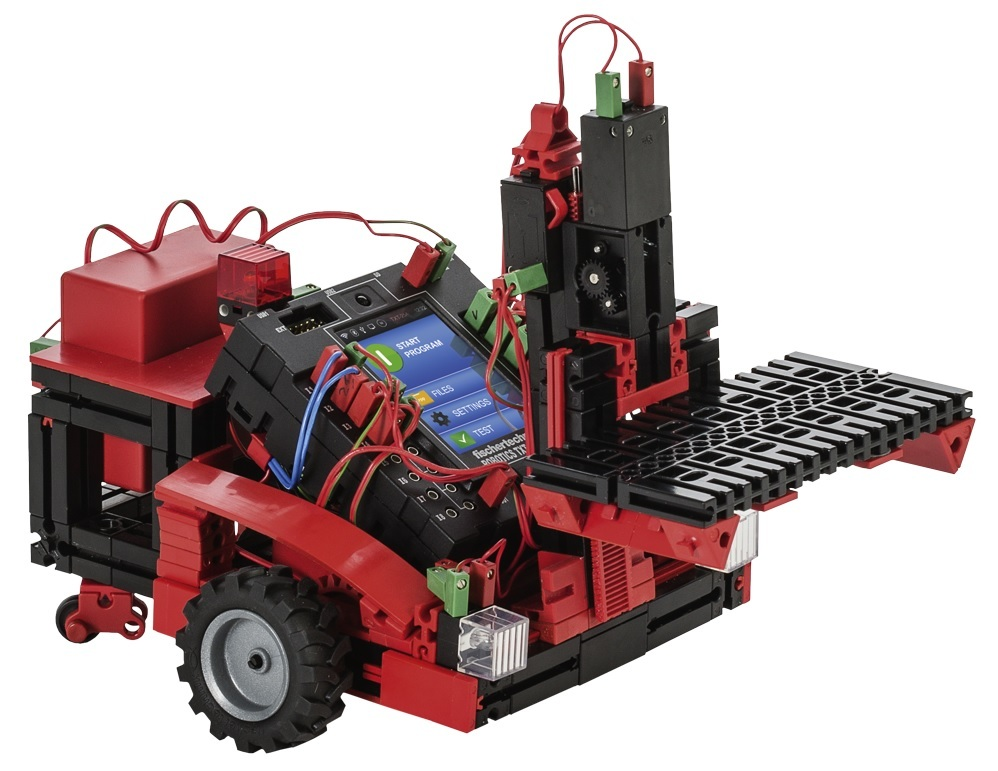
\includegraphics[width=300px]{images/fischertechnik_ROBO-TX-Explorer_02.jpg}
%			\caption[Fischertechnik - ROBO TX Explorer]{Fischertechnik - ROBO TX Explorer \footnotemark}
%		\label{fig:fischertechnik_ROBO-TX-Explorer}
%	\end{figure}
%	\footnotetext{Zdroj: \url{http://www.helago-cz.cz/eshop-519143-workstation-robo-tx-training-lab-tx-explorer-146560.html}}
%}

\begin{figure}[h]
 	\centering
	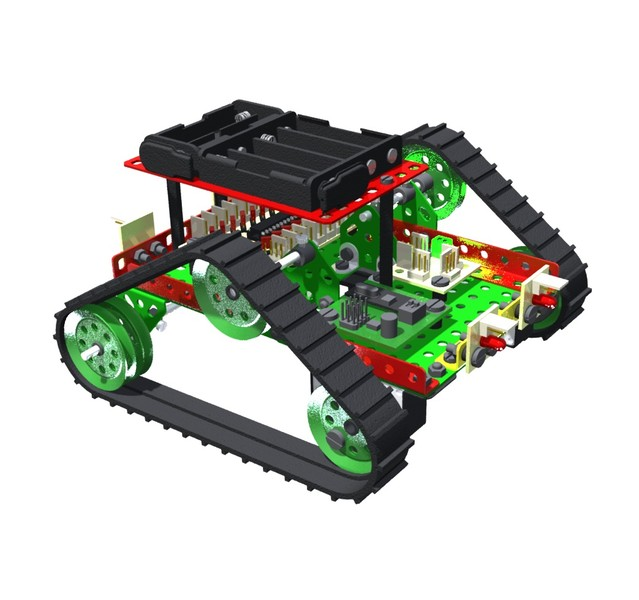
\includegraphics[width=250px]{images/MERKUR_Pasovy-podvozek-01_ATMEL+RC.jpg}
		\caption[MERKUR -- Pásový podvozek 01 -- ATMEL + RC]{MERKUR -- Pásový podvozek 01 -- ATMEL + RC\protect\footnotemark}
	\label{fig:MERKUR_Pasovy-podvozek-01_ATMEL+RC}
\end{figure}

\footnotetext{Zdroj: \url{http://www.merkurtoys.cz/vyrobky/pasovy-podvozek-merkur-s-elektronikou-rc}} 

Další zajímavou robotickou stavebnicí jsou Robotické sety od \merkur{u} \cite{merkur_roboticsSetsEshop}. 
Nabídka jednotlivých setů je relativně široka a v porovnání s \legoM{ }nebo \fischerT{ }nabízí ještě bližší kontakt s elektronikou a samotným hardwarem. 
Jako řídící mikrokontroléry můžete využít PIC nebo megaAVR od firmy Microchip. 
Vzhledem k použitým procesorům je možné tyto stroje programovat v C/C++, PICAXE BASIC nebo i grafickém prostředí \cite{picaxeCz_BlocklyForPICAXE}. 
Robotické stavebnice od Merkuru mají podobné 'problémy' jako \fischerT. 
Kladou na uživatele větší nároky, nemají tak zvučnou značku, mají omezenější základní sadu senzorů a neumožňují tak rychlou stavbu fungujícího robota.

Na závěr lze zmínit výukové roboty, kteří jsou primárně, na rozdíl od robotických stavebnic, zaměřeny na velmi úzkou oblast činnost (jízda po čáře, jednoduché sekvenční úkoly). 
Tito roboti jsou zajímavé z pohledu ceny, ale i případného jednoduššího využití ve výuce (žáci nemusí sestavovat konstrukci a hardware je plně připraven k používání). 
Naopak již neumožňují rozvoj kreativity studentů při stavbě a přizpůsobení robota pro různé soutěže (většinou je lze využívat jen v jedné soutěžní kategorii).  
Mezi takovéto roboty patři například Pololu 3pi \cite{robotPololu3pi} (primárně určen pro jízdu po čáře -- zvládá jezdit až 1 m/s) nebo Edison \cite{robotEdison} (umí jezdit po čáře, lze jej programovat graficky i v Pythonu, má různé senzory, je možné jej kombinovat s LEGEM). 
Tito roboti ovšem neumožňují takový rozsah činností jako \legoM.

\begin{figure}[h]
	\begin{minipage}[b]{.5\textwidth}
		\centering
		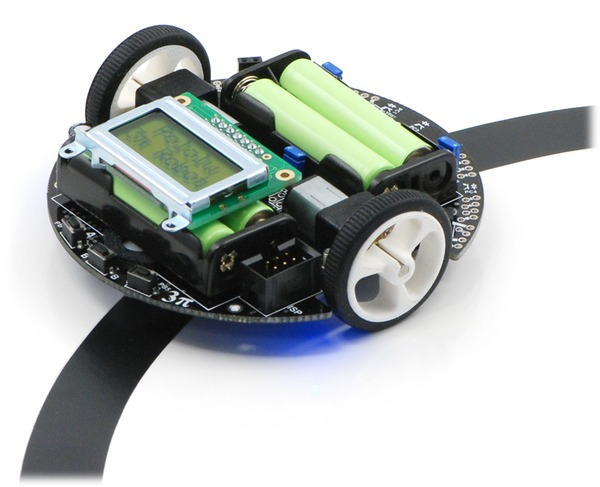
\includegraphics[width=\textwidth]{images/pololu-3pi-robot-8-on-line.jpg}
		\caption[Robot Pololu 3pi]{Robot Pololu 3pi\protect\footnotemark}
		\label{fig:pololu-3pi-robot-8-on-line}
	\end{minipage}
	\hfill
	\begin{minipage}[b]{.5\textwidth}
		\centering
		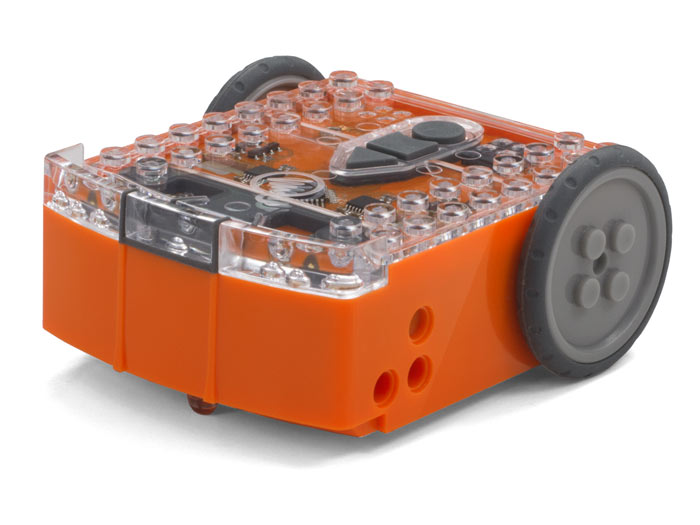
\includegraphics[width=\textwidth]{images/Edison-Educational-robot.jpg}
		\caption[Robot Edison]{Robot Edison\protect\footnotemark}
		\label{fig:Edison-Educational-robot}
	\end{minipage}
\end{figure}

\footnotetext{Zdroj: \url{https://www.pololu.com/product/975}} 
\footnotetext{Zdroj: \url{https://meetedison.com/meet-edison-v2-0/}} 

% putting two images beside each other
% source: http://tex.stackexchange.com/a/148445

%\begin{figure}[!tbp]
%	\begin{subfigure}[b]{.5\textwidth}
%		\centering
%		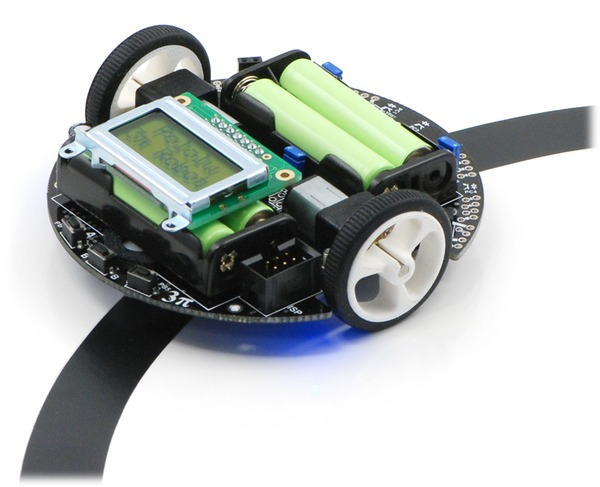
\includegraphics[width=\textwidth]{images/pololu-3pi-robot-8-on-line.jpg}
%		\caption[Robot Pololu 3pi]{Robot Pololu 3pi\protect\footnotemark}
%		\label{fig:pololu-3pi-robot-8-on-line}
%	\end{subfigure}
%	\hfill
%	\begin{subfigure}[b]{.5\textwidth}
%		\centering
%		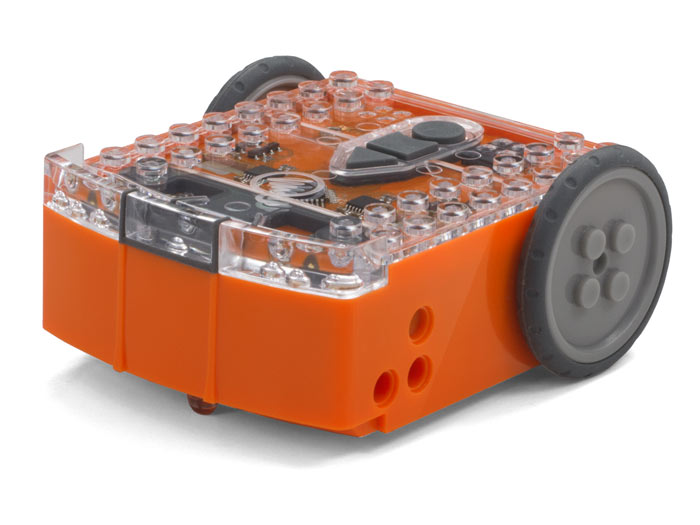
\includegraphics[width=\textwidth]{images/Edison-Educational-robot.jpg}
%		\caption[Robot Edison]{Robot Edison\protect\footnotemark}
%		\label{fig:Edison-Educational-robot}
%	\end{subfigure}
%	\caption{Roboti se zaměřením na velmi úzkou oblast činnost}
%\end{figure}
%
%\footnotetext{Zdroj: \url{https://www.pololu.com/product/975}} 
%\footnotetext{Zdroj: \url{https://meetedison.com/meet-edison-v2-0/}} 

\section{Historie LEGO MINDSTORMS}

Robotický set LEGO

